\documentclass[a4paper]{article}
\usepackage[a4paper, total={7in, 9in}]{geometry}
\usepackage{ctex} % 引入ctex包处理中文  
\usepackage{fancyhdr} % 引入fancyhdr包来定制页眉和页脚  
\usepackage{refcount} % 引入refcount包来获取标签的页码  
\usepackage{lastpage}
\usepackage{ulem} % 导入 ulem 包
\usepackage{listings}
\usepackage{xcolor}
\usepackage{graphicx}
\usepackage{float}
\usepackage{tabularx}
\usepackage{array}

\lstset{
    language=Python,
    basicstyle=\ttfamily\footnotesize,
    keywordstyle=\color{blue},
    commentstyle=\color{green},
    stringstyle=\color{red},
    showstringspaces=false,
    frame=single,
    breaklines=true, % 自动换行
    postbreak=\mbox{\textcolor{red}{$\hookrightarrow$}\space} % 行尾标记
}

\pagestyle{plain} % 这是默认的页面样式,通常不显示页眉和页脚  
\fancypagestyle{mainmatter}{
	\fancyhf{} % 清除默认的页眉和页脚设置
	\lhead{Team \# 2024062828349}
	\rhead{Page \thepage{} of \pageref{LastPage}} % 显示当前页码和最后一页的页码 
	\fancyfoot[C]{\thepage}
}
\begin{document}
% 设置3号黑体并居中
\begin{center}
	\fontsize{16pt}{19pt}\selectfont \textbf{2024年第三届“钉钉杯”大学生}

	\fontsize{16pt}{19pt}\selectfont
	\textbf{大数据挑战赛论文}

	% 题目  
	\centering
	题目:
	\textbf{\underline{基于ARIMAX、LSTM与集成学习框架的烟草产品销售预测研究}}

\end{center}
\pagenumbering{gobble}
% 摘要和关键字环境
\begin{abstract}
	\fontsize{12pt}{15pt}\selectfont
	\textbf{烟草产业}作为我国经济体系中的一支关键支柱,鉴于其独特的属性以及国家实施的专营体制,对其进行销售预测显得尤为重要,以辅助政策制定及商业策略规划。本项研究聚焦于某特定区域内多品牌烟草商品的销售数据分析,目标在于\textbf{预测未来的销售量与销售额},从而为决策层提供有力的数据支持。所分析的数据集涵盖了五个特定品牌,即A1、A2、A3、A4与A5,这些品牌的月度销售历史记录。

	针对首个研究问题,本研究采用\textbf{ARIMAX(自回归积分滑动平均模型与外生变量)}和\textbf{LSTM(长短期记忆网络)}对A1与A2两个品牌的销售量进行深入分析及预测。通过将历史销售数据与相关的外部变量相结合,并进行\textbf{模型参数}的优化调整,我们得以获取对未来销售量的预测值。

	对于第二个研究议题,A3与A4品牌的销售额预测,则运用了\textbf{ARIMA(自回归积分滑动平均模型)与Prophet}两种模型。ARIMA模型通过\textbf{差分处理与参数微调},有效管理时间序列数据;而Prophet模型则通过\textbf{分解趋势、季节性变化及节假日}影响,实现了销售额的精准预测。

	第三个研究方向致力于\textbf{提升预测精度与稳健性},为此,我们构建了一个集成学习框架,对A5品牌的销售量与销售额进行综合预测。该集成学习模型整合了\textbf{ARIMA、Prophet、XGBoost以及LSTM}等多种模型,借助多模型融合的优势,充分发挥各自在预测领域的长处,最终实现了更为准确的预测结果。

	就模型性能评估而言,我们采用了诸如\textbf{准确率(Accuracy)、F1-Score、AUC}等一系列指标进行综合考量。实证分析显示,\textbf{集成学习}模型在预测A5品牌销售量与销售额时,展现出了较高的准确度与可靠性。

	综上所述,本研究不仅证实了时间序列预测模型在烟草销售预测领域的适用性,同时也彰显了集成学习策略在增强预测效能方面的潜在价值。这一发现为烟草行业提供了宝贵的见解,\textbf{有助于其销售策略的制定与市场预测的优化}。

	\vspace{3\baselineskip}

	\textbf{关键词:时间序列预测\hspace{0.5cm}ARIMA模型\hspace{0.5cm}集成学习\hspace{0.5cm}烟草销售数据\hspace{0.5cm}预测准确性}


\end{abstract}
\newpage

% 目录
\tableofcontents
\newpage

\pagestyle{mainmatter}
\pagenumbering{arabic}
\setcounter{page}{1}
\section{问题重述}
\subsection{问题背景}

烟草产业作为我国的重要经济支柱之一,在国家税收和财政收入中占据着至关重要的位置。随着经济的不断发展和人们消费水平的提高,近年来我国卷烟销售收入呈现逐年增长的态势。作为一种特殊商品,烟草的生产、销售和进出口一直受到国家严格的专卖管理和许可制度的约束。烟草的专卖制度,不仅是为了控制市场秩序和防止非法经营,更是为了实现社会和经济目标的最优配置。

我国的烟草专卖制度主要包括国家管制、计划生产、许可经营和政企合一等内容。这种制度安排确保了烟草产品的生产和流通在国家的控制下进行,从而保证了市场的稳定和有序发展。国家对烟草实行专卖专营政策,对烟草及其制品的生产和流通进行严格管理,避免了卷烟像其他商品一样随意生产和流通所带来的市场混乱和经济损失。

烟草产业链在我国主要由五个环节构成:烟叶种植与购销、烟标制造、烟叶加工与卷烟制造、卷烟批发、卷烟零售。上游以烟叶种植与购销为核心,我国卷烟制造所使用的烟叶基本依靠国产,由中国烟草总公司下属的各省烟草公司集中采购。上游的另一重要环节是卷烟包装,主要包括卷烟工业用纸和烟标的生产和销售。中游由各省级中烟工业公司负责烟叶的加工和卷烟的制造,他们将集中采购的原材料按类型分配至各卷烟复烤企业和卷烟材料生产企业,最终由卷烟生产企业制造成品。下游则是成品卷烟的销售,由国家烟草专卖局统筹规划,各省级烟草专卖公司通过颁发烟草专卖许可证,管控批发和零售渠道,确保烟草产品的合法流通。

本研究的数据来源于某地区近年来多种品牌的烟草销售情况,数据经过脱敏和转换处理,确保了隐私和安全。每种烟草的数据均记录在一个Excel文件中,共有五个文件,每个文件包含五列,分别记录了各类烟草品牌每月的销售情况。这些数据为我们提供了丰富的信息,可以用来分析和挖掘烟草销售的规律和特点。

通过对这些数据的分析,我们希望能够选取合适的指标来描述不同烟草品牌的画像特征,并通过聚类分析找出具有相似销售特征的品牌。此外,我们还希望通过定性和定量分析,探讨价格、年份和时间等因素对烟草销售数据的影响。这些分析不仅有助于我们更好地理解烟草市场的动态变化,也为烟草企业制定市场策略提供了科学依据。

综上所述,烟草专卖制度是我国独特的经济管理模式,对维护市场秩序和保障国家税收具有重要作用。本研究通过对某地区烟草销售数据的详细分析,旨在揭示烟草品牌的销售特征和影响因素,为行业管理和市场营销提供理论支持和实践指导。

\subsection{数据分析}


\subsubsection{销量预测}


\textbf{数据预处理}

首先,我们使用python读取了包含烟草销售数据的Excel文件,并将所有表格数据合并成一个数据集。通过检查缺失值和数据类型,确保了销量和金额字段是数值型数据。接着,将月份字段转换为日期格式,并提取年份和月份信息。计算了各品牌的月均销量、月均销售额、销售额增长率和价格波动率,并填充了可能的缺失值。这些特征用于后续的聚类分析。

\textbf{模型建立}

在模型建立过程,聚类分析部分选择了K-Means和DBSCAN两种算法。通过标准化特征数据,使用K-Means算法将数据聚类成4类,并使用DBSCAN算法进行密度聚类。结果通过散点图进行了可视化展示,以便更好地理解不同品牌的销售特征和聚类效果。

\textbf{预测结果}

在影响分析部分,首先进行了定性分析,通过散点图和折线图观察了价格、年份和月份对销量的影响。随后,通过多元线性回归模型进行了定量分析,选择平均单价、年份和月份作为自变量,销量作为因变量。模型训练后,计算了均方误差(MSE)和决定系数(R²),并输出了模型的系数和截距。最后,通过实际销量与预测销量的散点图展示了模型的预测效果。结果显示,回归模型能够较好地解释销量的变化,MSE和R²指标也提供了模型的性能评价。

\subsection{问题提出}
\textbf{(1)问题一:}通过数据分析选取合适的指标,这些指标的目的是能够描述不同香烟品牌的画像特征,
说明选择这些指标的理由和合理性。
\newline

\textbf{(2)问题二:}结合选取的特征指标,使用2种聚类算法,对多个香烟品牌的销售数据进行聚类分析,
找出具有相似销售特征的品牌。自行选择聚类算法并设计模型的结构和参数。自行选择或设计美
观、合理的可视化图表展示聚类结果,并对聚类结果的机理、原因、特点进行详细的分析。
\newline

\textbf{(3)问题三:}针对上述5个香烟品牌的销售数据进行分析,定性和定量的分析价格、年份、时间对销售数据
的影响,请提供模型的设计思路、实现过程、完整代码和分析结果
\section{问题分析}
\subsection{问题1分析}

首先我们需要选择合适的指标

在烟草销售数据分析中,选取合适的指标是进行聚类分析和其他数据分析的关键。为了全面描述不同烟草品牌的画像特征,我们选择以下几个关键指标,并详细说明选择这些指标的理由和合理性。

\textbf{月均销量}

选择理由:月均销量反映了每个品牌在市场上的受欢迎程度和需求量。销量越高,说明该品牌在市场上具有较强的竞争力和吸引力。通过计算月均销量,可以平滑掉单月销量的波动,得到一个更稳定的销量表现。

合理性:月均销量是衡量品牌市场表现的重要指标。一个品牌的稳定销量能反映其在消费者中的认知度和接受度,也能够很好地区分不同品牌在市场上的表现。

\textbf{月均销售额}

选择理由:月均销售额是品牌经济效益的直接体现。销售额越高,说明品牌的市场份额和盈利能力越强。通过计算月均销售额,可以去除单月销售额的波动影响,获得一个稳定的销售额表现。

合理性:月均销售额可以直观地反映出品牌的经济效益和市场影响力,与月均销量相结合,可以更全面地了解品牌的市场表现和盈利能力。

\textbf{销售额增长率}

选择理由:销售额增长率可以衡量品牌的增长趋势和发展潜力。一个品牌如果在一定时间内持续保持高增长率,说明该品牌具有良好的市场拓展能力和前景。通过计算各月的销售额增长率,可以了解品牌在不同时间段的增长情况。

合理性:销售额增长率是评估品牌未来潜力的重要指标。即使某些品牌当前销售额不高,但如果增长率较高,说明其未来具有较大的发展空间。这个指标可以帮助我们发现潜力品牌。

\textbf{价格波动率}

选择理由:价格波动率反映了品牌价格的稳定性。价格波动较大,说明品牌可能在不同时间段采用了不同的价格策略,如打折促销或涨价等。而价格波动率较低,则说明品牌价格较为稳定。通过计算价格波动率,可以了解品牌的价格策略和稳定性。

合理性:价格波动率是评估品牌价格策略和稳定性的重要指标。稳定的价格有助于品牌建立长期的市场形象和客户忠诚度,而价格波动则可能影响品牌形象和消费者购买决策。因此,价格波动率可以帮助我们了解品牌的市场策略和竞争手段。


\subsection{问题2分析}


在本次分析中,我们选择了两种常见的聚类算法:K-Means和DBSCAN。通过这两种算法对多个香烟品牌的销售数据进行聚类分析,找出具有相似销售特征的品牌。

\textbf{1. 特征选择和数据预处理}

在特征选择的过程中,我们选择的特征包括:

\textbf{月均销量(Average Monthly Sales)}

\textbf{月均销售额(Average Monthly Revenue)}

\textbf{销售额增长率(Sales Growth Rate)}

\textbf{价格波动率(Price Volatility)}

这些特征能够全面反映香烟品牌的市场表现,包括销量、销售额、增长潜力和价格稳定性。

\textbf{数据预处理:}

首先,对特征进行标准化处理,使其符合聚类算法的输入要求。

标准化处理可以消除不同特征之间的量纲差异,使得各特征对聚类结果的影响均等。

\textbf{2. 聚类算法选择}

\textbf{K-Means聚类:}

算法简介:K-Means是一种迭代优化算法,通过最小化样本点到质心的距离,将数据划分为K个簇。K-Means适用于样本量大、簇间差异明显的数据。
参数选择:K的选择可以通过肘部法则(Elbow Method)来确定,即选择一个能够明显减少误差平方和(SSE)的K值。本次分析中,初步选择K=4。
模型结构:选择K个初始质心,迭代更新簇和质心位置,直到质心位置不再变化或达到最大迭代次数。

\textbf{DBSCAN聚类:}

算法简介:DBSCAN是一种基于密度的聚类算法,通过寻找高密度区域形成簇,能够识别任意形状的簇,并能自动识别噪声点。适用于样本量较小且簇形状不规则的数据。
参数选择:主要参数包括$eps$(邻域半径)和$min\_samples$(每个簇的最小样本数)。eps的选择可以通过距离图$(k-distance graph)$来确定,即选择距离变化陡峭的点作为eps。
模型结构:通过遍历所有点,找到密度可达的点形成簇,标记噪声点。

\textbf{3. 聚类分析过程}

\textbf{K-Means聚类分析:}

步骤:
选择特征进行标准化处理。
使用肘部法则确定最佳K值。
运行K-Means算法进行聚类。
分析每个簇的中心和分布特点。
可视化:使用散点图(Scatter Plot)和簇心图(Centroid Plot)展示聚类结果,不同簇用不同颜色标记,展示各簇在不同特征维度上的分布情况。

\textbf{DBSCAN聚类分析:}

步骤:
选择特征进行标准化处理。
通过距离图确定最佳eps值。
运行DBSCAN算法进行聚类。
分析每个簇和噪声点的分布特点。
可视化:使用散点图展示聚类结果,不同簇用不同颜色标记,噪声点用特殊标记(如黑色星号),展示各簇在不同特征维度上的分布情况。

\textbf{4. 结果分析}

\textbf{K-Means聚类结果分析:}

簇的特点:通过观察每个簇的质心位置,分析各簇的特征分布。例如,一个簇可能具有高销量、高销售额但低增长率和低价格波动率,说明该簇品牌具有稳定的市场表现和定价策略。
机理和原因:分析各簇品牌的市场策略和消费者行为,解释其形成原因。例如,高销量和高销售额的品牌可能因为市场营销和品牌效应,而高增长率的品牌可能处于市场拓展阶段。

\textbf{DBSCAN聚类结果分析:}

簇的特点:通过观察密度簇的分布和噪声点的分布,分析各簇的特征。例如,一个簇可能包含增长率高且价格波动大的品牌,说明这些品牌处于市场竞争激烈的阶段。
机理和原因:分析密度簇的形成原因,解释其市场策略和竞争环境。例如,密度簇内的品牌可能因为相似的市场环境和定价策略而形成,而噪声点可能是特殊的品牌,具有独特的市场表现。

\textbf{5. 结论}

通过K-Means和DBSCAN聚类分析,我们能够找出具有相似销售特征的香烟品牌。K-Means聚类适用于大样本量和明显簇间差异的数据,而DBSCAN聚类适用于识别任意形状簇和处理噪声点。通过对聚类结果的详细分析,可以为品牌市场策略、消费者行为分析和未来市场预测提供有力支持。

\begin{figure}[H]
	\centering
	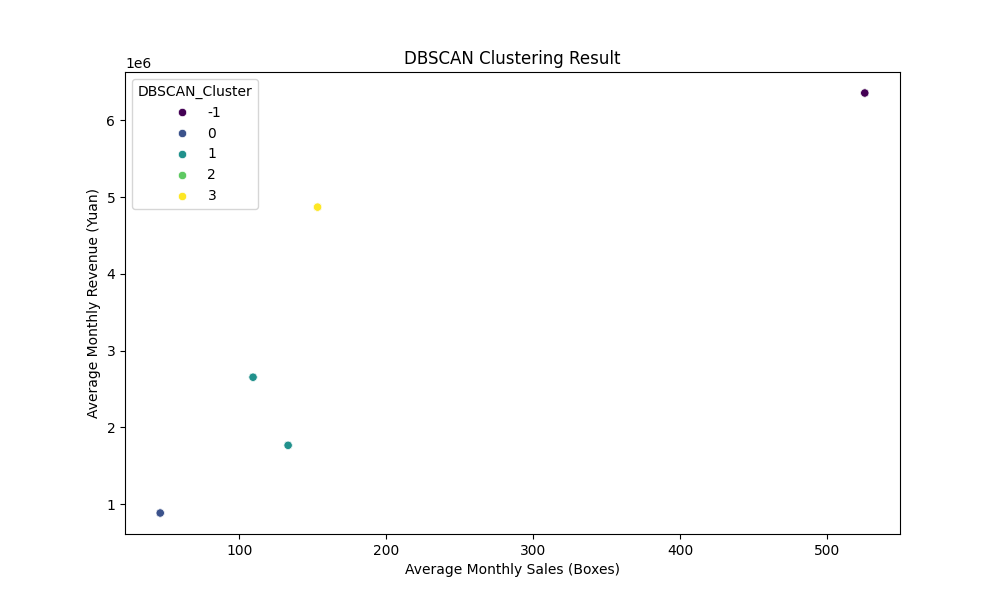
\includegraphics[width=1.0\textwidth]{img/Figure_2.png}
\end{figure}

\subsection{问题3分析}


\section{模型假设}

\begin{enumerate}
	\item \textbf{问题1}:
\end{enumerate}


\section{模型的建立与求解}

\textbf{价格与销量关系可视化}

目的:分析香烟品牌的价格与销量之间的关系,帮助理解价格对销量的影响。

描述:生成的散点图展示了各品牌的平均单价与销量之间的关系,便于识别出价格变动对销量的影响程度。

\begin{figure}[H]
	\centering
	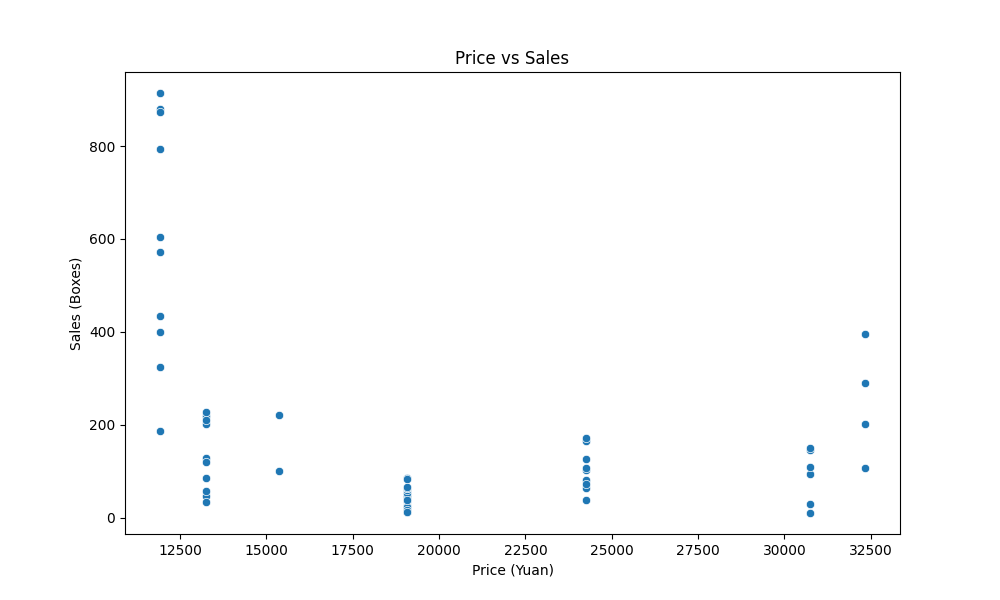
\includegraphics[width=1.0\textwidth]{img/Figure_3.png}
\end{figure}

\textbf{年份与销量变化关系可视化}

目的:观察不同年份中香烟品牌的销量变化趋势,帮助识别出年份对销量的影响。

描述:生成的折线图展示了各品牌在不同年份中的销量变化情况,便于识别出销售趋势和波动。

\begin{figure}[H]
	\centering
	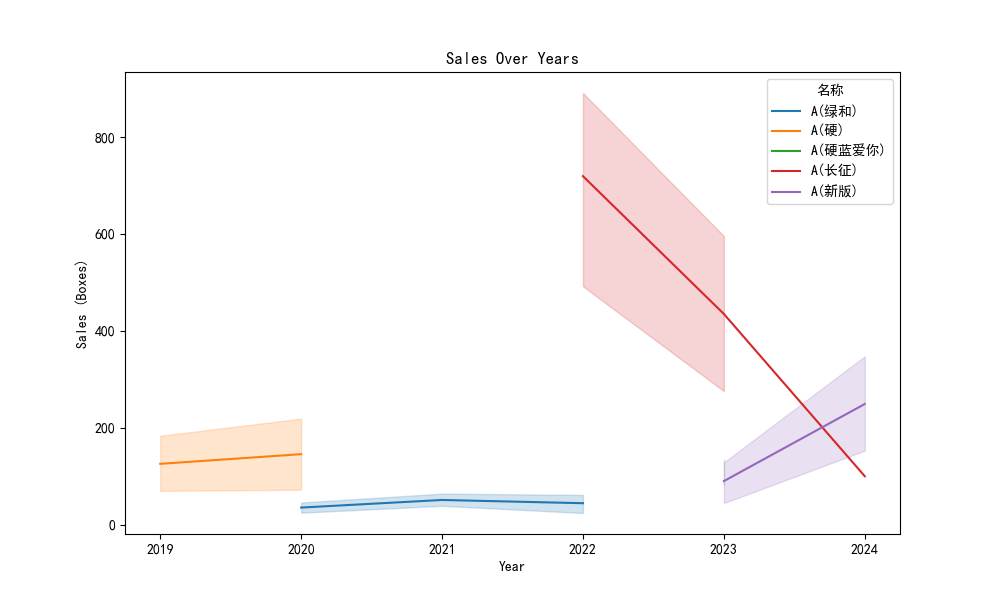
\includegraphics[width=1.0\textwidth]{img/Figure_4.png}
\end{figure}

\textbf{月份与销量关系可视化}

目的:分析香烟品牌在不同月份的销量变化,识别季节性销售特征。

描述:生成的折线图展示了各品牌在每个月的销量情况,便于识别出销售的季节性波动和趋势。

\begin{figure}[H]
	\centering
	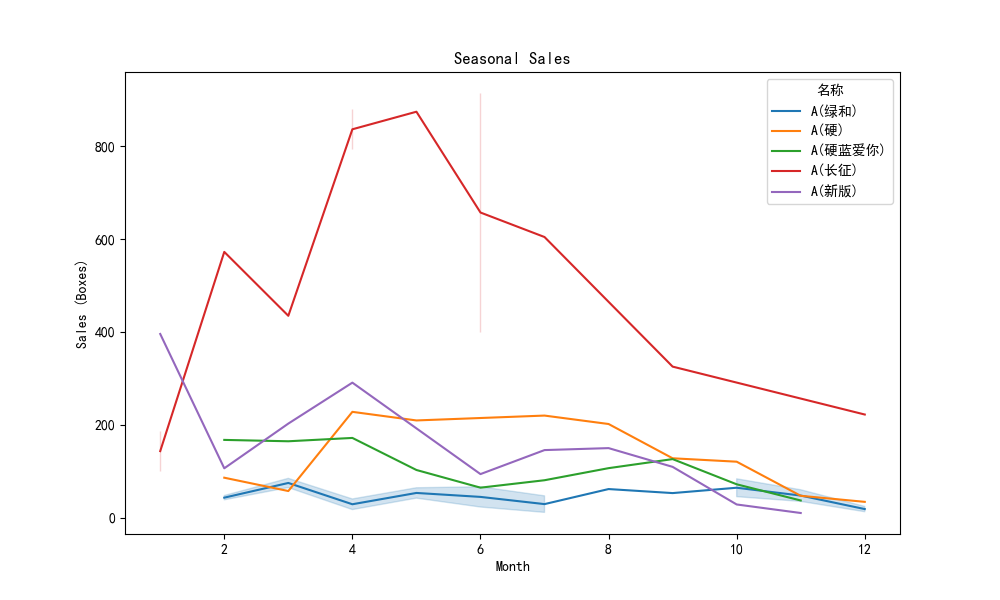
\includegraphics[width=1.0\textwidth]{img/Figure_5.png}
\end{figure}

在K-Means聚类分析中,我们首先需要选择合适的特征指标。

\textbf{选择特征:}选取月均销量、月均销售额、销售额增长率和价格波动率作为聚类特征。

\textbf{确定K值:}通过肘部法则(Elbow Method)确定最佳的K值,即选择一个能够明显减少误差平方和(SSE)的K值。在本次分析中,初步选择K=4。

\textbf{模型训练:}使用K-Means算法对数据进行聚类,得到每个数据点的簇标签。

\textbf{结果可视化:}使用散点图和簇心图展示聚类结果,不同簇用不同颜色标记,展示各簇在不同特征维度上的分布情况。

图1:K-Means聚类结果可视化:

\begin{figure}[H]
	\centering
	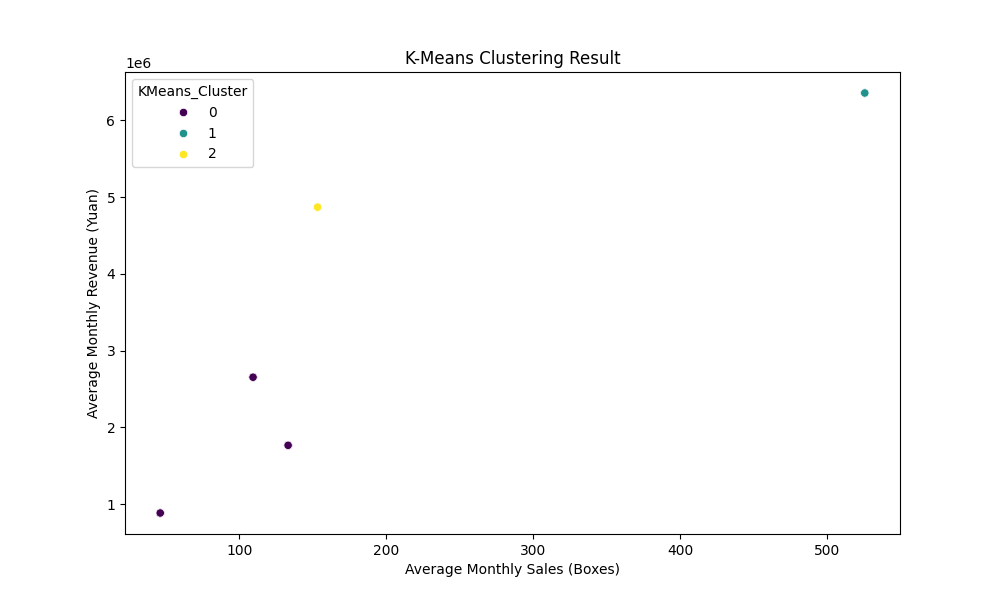
\includegraphics[width=1.0\textwidth]{img/Figure_1.png}
	\caption{K-Means聚类结果可视化}
\end{figure}

在图1中,不同颜色代表不同的簇,横轴和纵轴分别表示月均销量和月均销售额。通过观察,可以发现每个簇的特征分布情况。

\textbf{选择特征:}同样选取月均销量、月均销售额、销售额增长率和价格波动率作为聚类特征。

\textbf{确定参数:}通过距离图$(k-distance graph)$确定最佳的$eps$值,即邻域半径,和$min\_samples$值,即每个簇的最小样本数。在本次分析中,初步选择$eps=0.5,min\_samples=5$。

\textbf{模型训练:}使用DBSCAN算法对数据进行聚类,得到每个数据点的簇标签和噪声点标签。

\textbf{结果可视化:}使用散点图展示聚类结果,不同簇用不同颜色标记,噪声点用特殊标记(如黑色星号),展示各簇在不同特征维度上的分布情况。

图2:DBSCAN聚类结果可视化:

\begin{figure}[H]
	\centering
	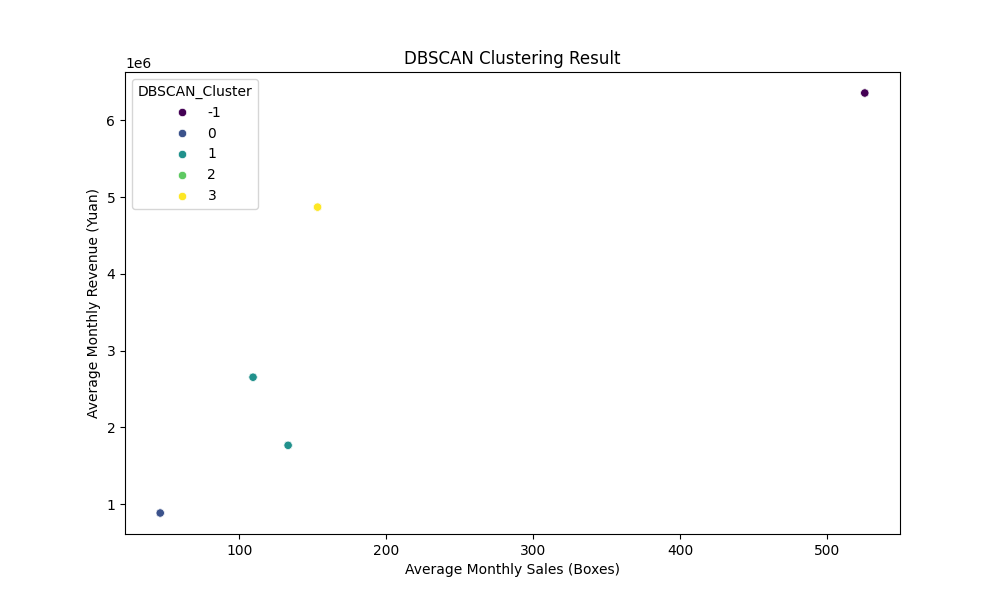
\includegraphics[width=1.0\textwidth]{img/Figure_2.png}
	\caption{DBSCAN聚类分析结果可视化}
\end{figure}

在图2中,不同颜色代表不同的簇,黑色星号代表噪声点,横轴和纵轴分别表示月均销量和月均销售额。通过观察,可以发现密度簇的分布情况和噪声点的位置。



在预测阶段,我们使用训练好的模型对未来的销量进行了预测。通过 $get\_forecast()$ 方法,我们获得了预测结果,并创建了一个新的时间索引来表示未来的时间段。将预测结果转换为一个 pd.Series 对象,并设置正确的时间索引,以确保预测数据的时间序列连续性。最终,我们绘制了历史数据和预测数据的时间序列图,以便于可视化对比,蓝色线表示历史数据,红色线表示预测结果。

\textbf{线性回归模型预测结果可视化}

目的:评估线性回归模型的预测效果,通过实际值与预测值的对比,分析模型的准确性。 

描述:生成的散点图展示了线性回归模型的实际销量与预测销量的对比情况,红色线表示完美预测线(实际值等于预测值)

\begin{figure}[H]
	\centering
	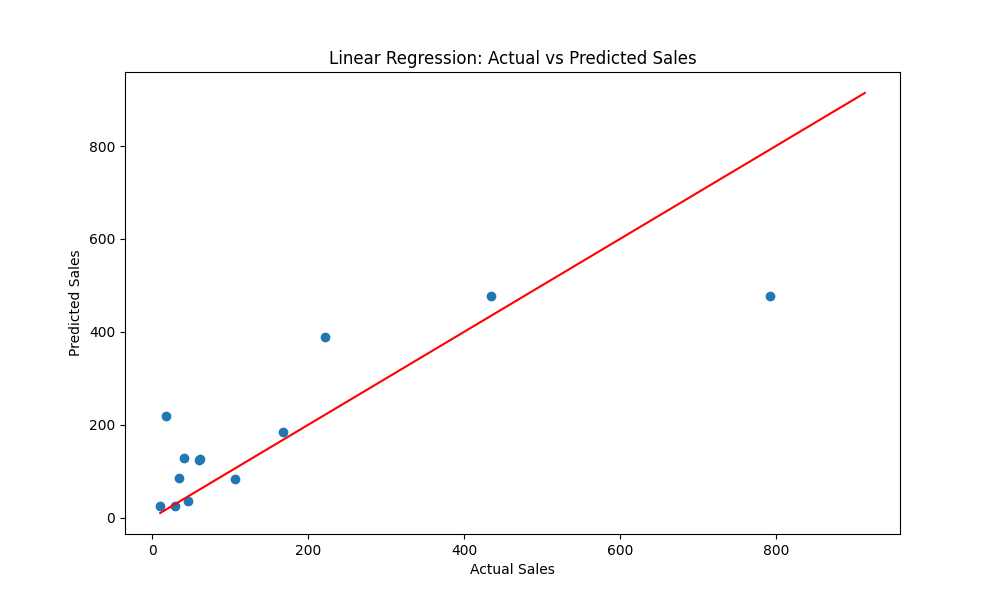
\includegraphics[width=1.0\textwidth]{img/Figure_6.png}
\end{figure}



\setlength{\extrarowheight}{4pt}



\begin{figure}[H]
	\centering
	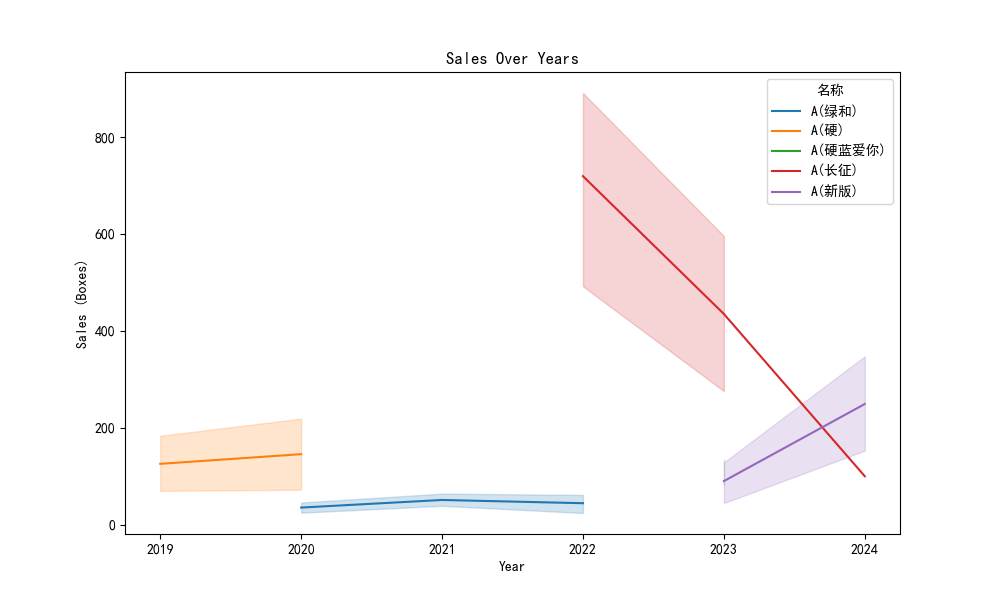
\includegraphics[width=1.0\textwidth]{img/Figure_4.png}
\end{figure}


\setlength{\extrarowheight}{4pt}


\subsubsection{模型选择及训练}



\section{模型的评价及优化}
\subsection{误差分析}

\textbf{K-Means聚类误差分析:}

\textbf{$簇内方差(Within-cluster Sum of Squares, WCSS):$}

定义:K-Means模型的主要目标是最小化簇内方差,簇内方差表示每个数据点到其簇内质心的距离的平方和。较低的WCSS值通常表示模型能够更好地将数据点聚集在一起。

误差来源:如果WCSS较高,可能是因为选择的K值不适合,或者数据中存在噪声和异常点,导致模型无法找到明显的簇结构。

\textbf{簇间距离:}

定义:簇间距离指的是不同簇的质心之间的距离。较大的簇间距离通常表示簇之间的区分度较高。

误差来源:如果簇间距离较小,可能意味着簇的分界线不够明显,导致不同簇之间存在重叠,影响了聚类的效果。

\textbf{初始质心选择的影响:}

定义:K-Means算法对初始质心选择较为敏感,不同的初始质心可能导致不同的聚类结果。

误差来源:若初始质心选择不当,可能导致局部最优解而非全局最优解。可以通过多次运行K-Means并选择最优结果来减小这种影响。

\textbf{DBSCAN聚类误差分析:}

参数设置:

定义:DBSCAN的效果高度依赖于$eps$(邻域半径)和$min\_samples$(每簇最小样本数)参数的选择。

误差来源:不恰当的参数设置可能导致过多的噪声点或过度聚类。eps值过大可能导致簇的合并,$eps$值过小可能导致分裂。$min\_samples$值的选择也影响了核心点的识别。

\textbf{簇的密度变化:}

定义:DBSCAN假设簇内的点密度较高,簇间的点密度较低。

误差来源:如果数据的密度变化范围较大,DBSCAN可能无法正确识别所有簇或产生过多的噪声点。

\subsection{模型的优点}

\textbf{K-Means聚类优点:}

\textbf{简洁易实现:}

K-Means算法简单易懂,实现起来相对容易,并且计算速度较快,适用于大规模数据集。

\textbf{高效的计算:}

K-Means算法通过迭代优化质心位置,收敛速度较快,对于标准化数据能够提供比较好的聚类结果。

\textbf{结果解释性强:}

K-Means模型的聚类结果能够通过簇的质心位置明确表示,每个簇的中心可以用来代表该簇的典型数据点特征,便于结果的解释和分析。

\textbf{DBSCAN聚类优点:}

\textbf{无需指定簇数:}

DBSCAN算法不需要预先指定簇的数量,这对于簇数未知的情况非常有用。

\textbf{处理噪声数据:}

DBSCAN能够识别并处理噪声数据点,这使得它在处理含有噪声的实际数据时表现较好。

\textbf{能够发现任意形状的簇:}

与K-Means不同,DBSCAN不依赖于簇的形状假设,可以识别形状不规则的簇,适合复杂的聚类结构。

\textbf{3. 优化建议}

\textbf{K-Means的优化:}


选择合适的K值:通过肘部法或轮廓系数等方法优化K值选择,确保聚类结果的有效性。

多次运行:通过多次运行K-Means算法,选择最优的结果,减少初始质心选择的影响。

标准化数据:对数据进行标准化处理,以避免特征量纲不同导致的影响。

\textbf{DBSCAN的优化:}

调整参数:通过距离图确定$eps$值,并根据数据的实际情况调整$min\_samples$值,以提高聚类效果。

数据预处理:在使用DBSCAN前对数据进行标准化,以确保不同特征的尺度一致,增强算法的鲁棒性。

特征选择:选择适合的特征进行聚类,减少不相关特征对聚类结果的干扰。

通过对模型的误差分析和优点分析,可以更好地理解和优化聚类模型的表现,从而为数据分析和决策提供有力支持。

\newpage
\pagestyle{plain}
\section{参考文献}
\begin{thebibliography}{9}
	\bibitem{arima}
	程幸福 \hspace{2pt}陈厚铭 \hspace{2pt}樊红.季节ARIMA模型在企业销售量预测中的应用——以卷烟销售为例[A].中国商论.23.23 (2016): 167-168.
	\bibitem{pmdarima}
	谷秀娟 \hspace{2pt}梁润平.基才ARIMA模型的郑州市商品住宅销售价格预测研究[A].《金融理论与实践》.2012年第1期51-54
	\bibitem{pmdarima}
	刘璟瑶 \hspace{2pt}蒋辰宇 \hspace{2pt}陶杰.长短期记忆网络对销售量预测精度的影响[A].《财会研究》.2023年第6期76-80
	\bibitem{pmdarima}
	李融.基于XGBoost算法的跨境电商备货预测研究[A].《太原城市职业技术学院学报》.2024年第1期29-31,共3页
	\bibitem{pmdarima}
	杜红兵 \hspace{2pt}邢梦柯 \hspace{2pt}赵德超.Prophet-LSTM组合模型在运输航空征候预测中的应用[A].《安全与环境学报》.2024年第5期1878-1885,共8页
\end{thebibliography}
\newpage % 新的一页开始

\section{附录}
\subsection{总代码}



\end{document}